% -*- latex -*-

\chapter{New Worklet Types}
\label{chap:NewWorkletTypes}

\index{worklet types!creating new|(}

The basic building block for an algorithm in \VTKm is the worklet.
Chapter~\ref{chap:Worklets} describes the different types of worklet types provided by \VTKm and how to use them to create algorithms.
However, it is entirely possible that this set of worklet types does not directly cover what is needed to implement a particular algorithm.
One way around this problem is to use some of the numerous back doors provided by \VTKm to provide less restricted access in the execution environment such as using whole arrays for random access.

However, it make come to pass that you encounter a particular pattern of execution that you find useful for implementing several algorithms.
If such is the case, it can be worthwhile to create a new worklet type that directly supports such a pattern.
Creating a new worklet type can provide two key advantages.
First, it makes implementing algorithms of this nature easier, which saves developer time.
Second, it can make the implementation of such algorithms safer.
By encapsulating the management of structures and regulating the data access, users of the worklet type can be more assured of correct behavior.

This chapter documents the process for creating new worklet types.
The operation of a worklet requires the coordination of several different object types such as dispatchers, argument handlers, and thread indices.
This chapter will provide examples of all these required components.
To tie all these features together, we start this chapter with a motivating example for an implementation of a custom worklet type.
The chapter then discusses the individual components of the worklet, which in the end come together for the worklet type that is then demonstrated.

\section{Motivating Example}
\label{sec:NewWorkletTypes:MotivatingExample}

For our motivation to create a new worklet type, let us consider the use case of building fractals.
Fractals are generally not a primary concern of visualization libraries like \VTKm, but building a fractal (or approximations of fractals) has similarities the the computational geometry problems in scientific visualization.
In particular, we consider the class of fractals that is generated by replacing each line in a shape with some collection of lines.
These types of fractals are interesting because, in addition to other reasons, the right parameters result in a shape that has infinite length confined to a finite area.

A simple but well known example of a line fractal is the \index{Koch Snowflake}Koch Snowflake.
The Koch Snowflake starts as a line or triangle that gets replaced with the curve shown in Figure~\ref{fig:KochShape}.

\begin{figure}[htb]
  \centering
  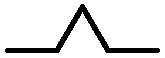
\includegraphics[scale=2]{images/Koch1.pdf}
  \caption{Basic shape for the Koch Snowflake.}
  \label{fig:KochShape}
\end{figure}

The fractal is formed by iteratively replacing the curve's lines with this basic shape.
Figure~\ref{fig:KochIterations} shows the second iteration and then several subsequent iterations that create a ``fuzzy'' curve.
The curve is confined to a limited area regardless of how many iterations are performed, but the length of the curve approaches infinity as the number of iterations approaches infinity.

\begin{figure}[htb]
  \centering
  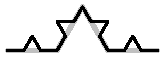
\includegraphics[scale=2]{images/Koch2.pdf}
  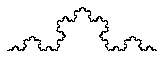
\includegraphics[scale=2]{images/Koch5.pdf}
  \caption[The Koch Snowflake after multiple iterations.]{
    The Koch Snowflake after the second iteration (left image) and after several more iterations (right image).
  }
  \label{fig:KochIterations}
\end{figure}

In our finite world we want to estimate the curve of the Koch Snowflake by performing a finite amount of iterations.
This is similar to a \index{Lindenmayer system}Lindenmayer system but with less formality.
The size of the curve grows quickly and in practice it takes few iterations to make close approximations.

\begin{didyouknow}
  The Koch Snowflake is just one example of many line fractals we can make with this recursive line substitution, which is why it is fruitful to create a worklet type to implement such fractals.
  We use the Koch Snowflake to set up the example here.
  Section~\ref{sec:NewWorkletTypes:Using} provides several more examples.
\end{didyouknow}

To implement line fractals of this nature, we want to be able to define the lines of the base shape in terms of parametric coordinates and then transform the coordinates to align with a line segment.
For example, the Koch Snowflake base shape could be defined with parametric coordinates shown in Figure~\ref{fig:KochParametric}.

\begin{figure}[htb]
  \centering
  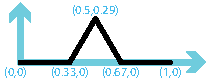
\includegraphics[scale=2]{images/KochParametric}
  \caption{Parametric coordinates for the Koch Snowflake shape.}
  \label{fig:KochParametric}
\end{figure}

Given these parametric coordinates, for each line we define an axis with the main axis along the line segment and the secondary axis perpendicular to that.
Given this definition, we can perform each fractal iteration by applying this transform for each line segment as shown in Figure~\ref{fig:KochApply}.

\begin{figure}[htb]
  \centering
  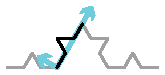
\includegraphics[scale=2]{images/KochApply}
  \caption{Applying the line fractal transform for the Koch Snowflake.}
  \label{fig:KochApply}
\end{figure}

To implement the application of the line fractal demonstrated in Figure~\ref{fig:KochApply}, let us define a class named \textcode{LineFractalTransform} that takes as its constructor the coordinates of two ends of the original line.
As its operator, \textcode{LineFractalTransform} takes a point in parametric space and returns the coordinates in world space in respect to the original line segment.
We define this class in the \vtkmexec{} namespace because the intended use case is by worklets of the type we are making.
A definition of \textcode{LineFractalTransform} is given in Example~\ref{ex:LineFractalTransform}

\vtkmlisting[ex:LineFractalTransform]{A support class for a line fractal worklet.}{LineFractalTransform.h}

\begin{didyouknow}
  The definition of \textcode{LineFractalTransform} (or something like it) is not strictly necessary for implementing a worklet type.
  However, it is common to implement such supporting classes that operate in the execution environment in support of the operations typically applied by the worklet type.
\end{didyouknow}

The remainder of this chapter is dedicated to defining a \textcode{WorkletLineFractal} class and supporting objects that allow you to easily make line fractals.
Example~\ref{ex:KochSnowflake} demonstrates how we intend to use this worklet type.

\vtkmlisting[ex:KochSnowflake]{Demonstration of how we want to use the line fractal worklet.}{KochSnowflake.cxx}

\section{Thread Indices}
\label{sec:ThreadIndices}

\index{thread indices|(}

The first internal support class for implementing a worklet type is a class that manages indices for a thread.
As the name would imply, the thread indices class holds a reference to an index identifying work to be done by the current thread.
This includes indices to the current input element and the current output element.
The thread indices object can also hold other information (that may not strictly be index data) about the input and output data.
For example, the thread indices object for topology maps (named \vtkmexecarg{ThreadIndicesTopologyMap}) maintains cell shape and connection indices for the current input object.

As is discussed briefly in Section~\ref{sec:Fetch}, a thread indices object is given to the \vtkmexecarg{Fetch} class to retrieve data from the execution object.
The thread indices object serves two important functions for the \textidentifier{Fetch}.
The first function is to cache information about the current thread that is likely to be used by multiple objects retrieving information.
For example, in a point to cell topology map data from point fields must be retrieved by looking up indices in the topology connections.
It is more efficient to retrieve the topology connections once and store them in the thread indices than it is to look them up independently for each field.

The second function of thread indices is to make it easier to find information about the input domain when fetching data.
Once again, getting point data in a point to cell topology map requires looking up connectivity information in the input domain.
However, the \textidentifier{Fetch} object for the point field does not have direct access to the data for the input domain.
Instead, it gets this information from the thread indices.

All worklet classes have a method named \textcode{GetThreadIndices} that constructs a thread indices object for a given thread.
\textcode{GetThreadIndices} is called with 5 parameters: a unique index for the thread (i.e. worklet instance), an array portal that maps output indices to input indices (which might not be one-to-one if a scatter is being used), an array portal that gives the visit index for each output index, the execution object for the input domain, and an offset of the current index of the local invoke to a global indexing (used for streaming).

The base worklet implementation provides an implementation of \textcode{GetThreadIndices} that creates a \vtkmexecarg{ThreadIndicesBasic} object.
This provides the minimum information required in a thread indices object, but non-trivial worklet types are likely to need to provide their own thread indices type.
This following example shows the implementation of \textcode{GetThreadIndices} we will use in our worklet type superclass (discussed in more detail in Section~\ref{sec:NewWorkletTypes:WorkletSuperclass}).

\vtkmlisting[ex:GetThreadIndices]{Implementation of \textcode{GetThreadIndices} in a worklet superclass.}{GetThreadIndices.cxx}

As we can see in Example~\ref{ex:GetThreadIndices}, our new worklet type needs a custom thread indices class.
Specifically, we want the thread indices class to manage the coordinate information of the input line segment.

\begin{didyouknow}
  The implementation of a thread indices object we demonstrate here stores point coordinate information in addition to actual indices.
  It is acceptable for a thread indices object to store data that are not strictly indices.
  That said, the thread indices object should only load data (index or not) that is almost certain to be used by any worklet implementation.
  The thread indices object is created before any time that the worklet operator is called.
  If the thread indices object loads data that is never used by a worklet, that is a waste.
\end{didyouknow}

An implementation of a thread indices object usually derives from \vtkmexecarg{ThreadIndicesBasic} (or some other existing thread indices class) and adds to it information specific to a particular worklet type.

\vtkmlisting{Implementation of a thread indices class.}{ThreadIndicesLineFractal.h}

\index{thread indices|)}

\section{Signature Tags}
\label{sec:NewWorkletTypes:SignatureTags}

It is common that when defining a new worklet type, the new worklet type is associated with new types of data.
Thus, it is common that implementing new worklet types involves defining custom tags for \controlsignature{}s and \executionsignature{}s.
This in turn typically requires creating custom \textidentifier{TypeCheck}, \textidentifier{Transport}, and \textidentifier{Fetch} classes.

Chapter~\ref{chap:WorkletArguments} describes in detail the process of defining new worklet types and the associated code to manage data from an argument to the dispatcher's \textcode{Invoke} to the data that are passed to the worklet operator.
Rather than repeat the discussion, readers should review Chapter~\ref{chap:WorkletArguments} for details on how custom arguments are defined for a new worklet type.
In particular, we use the code from Examples \ref{ex:TypeCheckTag2DCoordinates} (page \pageref{ex:TypeCheckTag2DCoordinates}), \ref{ex:TransportImpl} (page \pageref{ex:TransportImpl}), and \ref{ex:FetchImplBasic} (page \pageref{ex:FetchImplBasic}) to implement an argument representing 2D line segments (which is our input domain).
All these examples culminate in the definition of a \controlsignature tag in our worklet superclass.

\vtkmlisting{Custom \protect\controlsignature tag for the input domain of our example worklet type.}{WorkletLineFractalInputDomainTag.cxx}

As you have worked with different existing worklet types, you have likely noticed that different worklet types have special \executionsignature tags to point to information in the input domain.
For example, a point to cell topology map has special \executionsignature tags for getting the input cell shape and the indices to all points incident on the current input cell.
We described in the beginning of the chapter that we wanted our worklet type to provide worklet implementations an object named \textcode{LineFractalTransform} (Example~\ref{ex:LineFractalTransform}), so it makes sense to define our own custom \executionsignature tag to provide this object.

Chapter~\ref{chap:WorkletArguments} gives an example of a custom \executionsignature tag that modifies what information is fetched from an argument (Examples \ref{ex:AspectImpl} and \ref{ex:CustomExecutionSignatureTag}).
However, \executionsignature tags that only pull data from input domain behave a little differently because they only get information from the thread indices object and ignore the associated data object.
This is done by providing a partial specialization of \vtkmexecarg{Fetch} that specializes on the aspect tag but not on the fetch tag.

\vtkmlisting[ex:InputDomainFetch]{A \textidentifier{Fetch} for an aspect that does not depend on any control argument.}{InputDomainFetch.h}

The definition of an associated \executionsignature tag simply has to use the define aspect as its \textcode{AspectTag}.
The tag also has to define a \textcode{INDEX} member (which is required of all \executionsignature tags).
This is problematic as this execution argument does not depend on any particular control argument.
Thus, it is customary to simply set the \textcode{INDEX} to 1.
There is guaranteed to be at least one \controlsignature argument for any worklet implementation.
Thus, the first argument is sure to exist and can then be ignored.

\vtkmlisting{Custom \protect\executionsignature tag that only relies on input domain information in the thread indices.}{WorkletLineFractalTransformTag.cxx}

So far we have discussed how to get input line segments into our worklet.
We also need a \controlsignature tag to represent the output line segments created by instances of our worklet.
The motivating example has each worklet outputting a fixed number (greater than 1) of line segments for each input line segment.
To manage this, we will define another \controlsignature tag that outputs these line segments (as two \textidentifier{Vec}-2 coordinates).
This is defined as a \textidentifier{Vec} of \textidentifier{Vec}-2's.
The tag takes the number of line segments as a template argument.

\vtkmlisting[ex:WorkletLineFractalOutputTag]{Output \protect\controlsignature tag for our motivating example.}{WorkletLineFractalOutputTag.cxx}

You can see that the tag in Example~\ref{ex:WorkletLineFractalOutputTag} relies on a custom transport named \textcode{TransportTag2DLineSegmentsOut}.
There is nothing particularly special about this transport, but we provide the implementation here for completeness.

\vtkmlisting{Implementation of \textidentifier{Transport} for the output in our motivating example.}{TransportImpl2.h}

In addition to these special \controlsignature tags that are specific to the nature of our worklet type, it is common to need to replicate some more common or general \controlsignature tags.
One such tag, which is appropriate for our worklet type, is a ``field'' type that takes an array with exactly one value associated with each input or output element.
We can build these field tags using existing type checks, transports, and fetches.
The following example defines a \sigtag{FieldIn} tag for our fractal worklet type.
A \sigtag{FieldOut} tag can be made in a similar manner.

\vtkmlisting{Implementing a \textsignature{FieldIn} tag.}{WorkletLineFractalFieldInTag.cxx}


\section{Worklet Superclass}
\label{sec:NewWorkletTypes:WorkletSuperclass}
\label{sec:WorkletSuperclass}

The penultimate step in defining a new worklet type is to define a class that will serve as the superclass of all implementations of worklets of this type.
This class itself must inherit from \vtkmworkletinternal{WorkletBase}.
By convention the worklet superclass is placed in the \vtkmworklet{} namespace and its name starts with \textidentifier{Worklet}.

Within the worklet superclass we define the signature tags (as discussed in Section~\ref{sec:NewWorkletTypes:SignatureTags}) and the \textcode{GetThreadIndices} method (as discussed in Section~\ref{sec:ThreadIndices}.
The worklet superclass can also override other default behavior of the \textidentifier{WorkletBase} (such as special scatter).
And the worklet superclass can provide other items that might be particularly useful to its subclasses (such as commonly used tags).

\vtkmlisting[ex:WorkletSuperclass]{Superclass for a new type of worklet.}{WorkletLineFractal.h}

\begin{commonerrors}
  Be wary of creating worklet superclasses that are templated.
  The C++ compiler rules for superclass templates that are only partially specialized are non-intuitive.
  If a subclass does not fully resolve the template, features of the superclass such as signature tags will have to be qualified with \textcode{typename} keywords, which reduces the usability of the class.
\end{commonerrors}

\section{Dispatcher}
\label{sec:NewWorkletTypes:Dispatcher}

\index{dispatcher!creating new|(}

The final element required for a new worklet type is an associated dispatcher class for invoking the worklet.
As documented in Chapter~\ref{chap:Worklets}, each worklet type has its own associated dispatcher object.
By convention, the dispatcher is placed in the \vtkmworklet{} and has the same name as the worklet superclass with the \textidentifier{Worklet} replaced with \textidentifier{Dispatcher}.
So since the worklet superclass for our motivating example is named \textcode{WorkletLineFractal}, we name the associated dispatcher \textcode{DispatcherLineFractal}.

Also by convention, a dispatcher is a templated class.
The first template argument should be the type of the worklet (which should be a subclass of the associated worklet superclass).
The last template argument should be a device adapter tag with a default value set to \vtkmmacro{VTKM\_DEFAULT\_DEVICE\_ADAPTER\_TAG}.
Other template arguments that the dispatcher might need should be placed in between these two.

\vtkmlisting{Standard template arguments for a dispatcher class.}{DispatcherTemplate.cxx}

A dispatcher implementation inherits from \vtkmworkletinternal{DispatcherBase}.
\textidentifier{DispatcherBase} is itself a templated class with the following three templated arguments.
\begin{enumerate}
\item
  The dispatcher class that is subclassing \textidentifier{DispatcherBase}.
  All template arguments must be given.
\item
  The type of the worklet being dispatched (which by convention is the first argument of the dispatcher's template).
\item
  The expected superclass of the worklet, which is associated with the dispatcher implementation.
  \textidentifier{DispatcherBase} will check that the worklet has the appropriate superclass and provide a compile error if there is a mismatch.
\end{enumerate}

\begin{didyouknow}
  The convention of having a subclass be templated on the derived class' type is known as the Curiously Recurring Template Pattern (CRTP).
  In the case of \textidentifier{DispatcherBase}, \VTKm uses this CRTP behavior to allow the general implementation of \textcode{Invoke} to run \textcode{DoInvoke} in the subclass, which as we see in a moment is itself templated.
\end{didyouknow}

\vtkmlisting{Subclassing \textidentifier{DispatcherBase}.}{DispatcherSuperclass.cxx}

The constructor for the dispatcher should take as an argument an instance of the worklet to be invoked.
For convenience, this worklet argument should default to a new instance of the worklet.

\vtkmlisting{Typical constructor for a dispatcher.}{DispatcherConstructor.cxx}

Finally, the dispatcher must implement a const method named \textcode{DoInvoke}.
The \textcode{DoInvoke} method should take a single argument.
The argument will be an object of type \vtkminternal{Invocation} although it is usually more convenient to just express the argument type as a single template parameter.
The \textcode{Invocation} could contain several data items, so it is best to pass this argument as a constant reference.

\vtkmlisting{Declaration of \textcode{DoInvoke} of a dispatcher.}{DispatcherDoInvokePrototype.cxx}

\index{invocation object|(}
\index{dispatcher!invocation object|(}

\textidentifier{Invocation} is an object that encapsulates the state and data relevant to the invoke.
\textidentifier{Invocation} contains multiple types and data items.
For brevity only the ones most likely to be used in a \textcode{DoInvoke} method are documented here.
We discuss these briefly before getting back to the implementation of \textcode{DoInvoke}.

\vtkminternal{Invocation} contains a data member named \textcode{Parameters} that contains the data passed to the \textcode{Invoke} method of the dispatcher (with some possible transformations applied).
\textcode{Parameters} is stored in a \vtkminternal{FunctionInterface} template object.
(\textidentifier{FunctionInterface} is described in Chapter~\ref{chap:FunctionInterfaceObjects}.)
The specific type of \textcode{Parameters} is defined as type \textcode{ParameterInterface} in the \textidentifier{Invoke} object.

The \textidentifier{Invoke} object also contains the types \textcode{ControlInterface} and \textcode{ExecutionInterface} that are \textidentifier{FunctionInterface} classes built from the \controlsignature and \executionsignature of the worklet.
These \textidentifier{FunctionInterface} classes provide a simple mechanism for introspecting the arguments of the worklet's signatures.

All worklets must also define an input domain index, which points to one of the \controlsignature/\textidentifier{Invoke} arguments.
This number is also captured in the \vtkminternal{Invocation} object in a field named \textcode{InputDomainIndex}.
For convenience, \textidentifier{Invocation} also has the type \textcode{InputDomainTag} set to be the same as the \controlsignature argument corresponding to the input domain.
Likewise, \textidentifier{Invocation} has the type \textcode{InputDomainType} set to be the same type as the (transformed) input domain argument to \textcode{Invoke}.
\textidentifier{Invocation} also has a method name \textcode{GetInputDomain} that returns the invocation object passed to \textcode{Invoke}.

\index{dispatcher!invocation object|)}
\index{invocation object|)}

Getting back to the implementation of a dispatcher, the \textcode{DoInvoke} should first verify that the \controlsignature argument associated with the input domain is of the expected type.
This can be done by comparing the \textidentifier{Invocation}\textcode{::InputDomainTag} with the expected signature tag using a tool like \textcode{std::is\_same}.
This step is not strictly necessary, but is invaluable to users diagnosing issues with using the dispatcher.
It does not hurt to also check that the \textcode{Invoke} argument for the input domain is also the same as expected (by checking \textidentifier{Invocation}\textcode{::InputDomainType}).
It is additionally helpful to have a descriptive comment near these checks.

\vtkmlisting{Checking the input domain tag and type.}{CheckInputDomainType.cxx}

Next, \textcode{DoInvoke} must determine the size in number of elements of the input domain.
When the default identity scatter is used, the input domain size corresponds to the number of instances the worklet is executed.
(Other scatters will transform the input domain size to an output domain size, and that output domain size will determine the number of instances.)
The input domain size is generally determined by using \textidentifier{Invocation}::\textcode{::GetInputDomain} and querying the input domain argument.
In our motivating example, the input domain is an \textidentifier{ArrayHandle} and the input domain size is half the size of the array (since array entries are paired up into line segments).

The final thing \textcode{DoInvoke} does is call \textcode{BasicInvoke} on its \textidentifier{DispatcherBase} superclass.
\textcode{BasicInvoke} does the complicated work of transferring arguments, scheduling the parallel job, and calling the worklet's operator.
\textcode{BasicInvoke} takes three arguments: the \textidentifier{Invocation} object, the size of the input domain, and the device adapter tag to run on.

\vtkmlisting{Calling \textcode{BasicInvoke} from a dispatcher's \textcode{DoInvoke}.}{CallBasicInvoke.cxx}

Putting this all together, the following example demonstrates the full implementation of the dispatcher for our motivating example.

\vtkmlisting[ex:DispatcherImplementation]{Implementation of a dispatcher for a new type of worklet.}{DispatcherLineFractal.h}

\index{dispatcher!creating new|)}


\section{Using the Worklet}
\label{sec:NewWorkletTypes:Using}

Now that we have our full implementation of a worklet type that generates line fractals, let us have some fun with it.
The beginning of this chapter shows an implementation of the Koch Snowflake.
The remainder of this chapter demonstrates other fractals that are easily implemented with our worklet type.

\subsection{Quadratic Type 2 Curve}

There are multiple variants of the Koch Snowflake.
One simple but interesting version is the quadratic type 1 curve.
This fractal has a shape similar to what we used for Koch but has right angles and goes both up and down as shown in Figure~\ref{fig:QuadraticType2}.

\begin{figure}[htb]
  \centering
  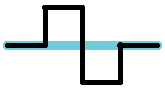
\includegraphics[scale=2]{images/QuadraticType2_1}
  \hfill
  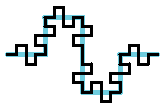
\includegraphics[scale=2]{images/QuadraticType2_2}
  \hfill
  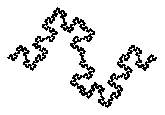
\includegraphics[scale=2]{images/QuadraticType2_4}
  \caption[The quadratic type 2 curve fractal.]{
    The quadratic type 2 curve fractal.
    The left image gives the first iteration.
    The middle image gives the second iteration.
    The right image gives the result after a few iterations.
  }
  \label{fig:QuadraticType2}
\end{figure}

The quadratic type 2 curve is implemented exactly like the Koch Snowflake except we output 8 lines to every input instead of 4, and, of course, the positions of the lines we generate are different.

\vtkmlisting{A worklet to generate a quadratic type 2 curve fractal.}{QuadraticType2.cxx}

\subsection{Tree Fractal}

Another type of fractal we can make is a tree fractal.
We will make a fractal similar to a Pythagoras tree except using lines instead of squares.
Our fractal will start with a vertical line that will be replaced with the off-center ``Y'' shape shown in Figure~\ref{fig:TreeFractal}.
Iterative replacing using this ``Y'' shape produces a bushy tree shape.

\begin{figure}[htb]
  \centering
  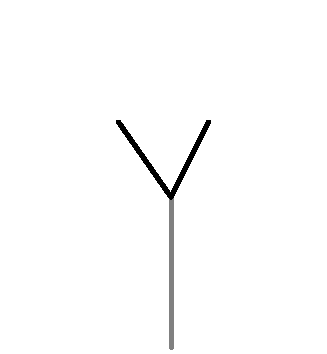
\includegraphics[scale=1]{images/Tree01}
  \hfill
  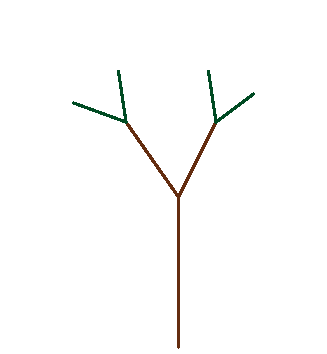
\includegraphics[scale=1]{images/Tree02}
  \hfill
  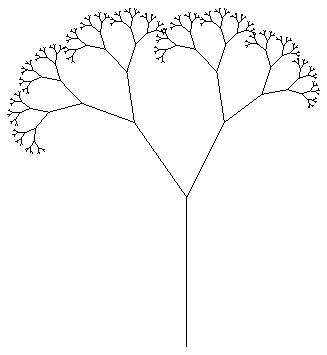
\includegraphics[scale=1]{images/Tree08}
  \caption[The tree fractal.]{
    The tree fractal replaces each line with the ``Y'' shape shown at left.
    An iteration grows branches at the end (middle).
    After several iterations the tree branches out to the bushy shape at right.
  }
  \label{fig:TreeFractal}
\end{figure}

One complication of implementing this tree fractal is that we really only want to apply the ``Y'' shape to the ``leaves'' of the tree.
For example, once we apply the ``Y'' to the trunk, we do not want to apply it to the trunk again.
If we were to apply it to the trunk again, we would create duplicates of the first layer of branches.

We can implement this feature in our worklet by using a count scatter.
(Worklet scatters are described in Section~\ref{sec:WorkletScatter}.)
Instead of directing the fractal worklet to generate 3 output line segments for every input line segment, we tell the fractal worklet to generate just 1 output line segment.
We then use a scatter counting to generate 3 line segments for the leaves and 1 line segment for all other line segments.
The count array for the initial iteration is initialized to a single 3.
Each iteration then creates the count array for the next iteration by writing a 1 for the base line segment and a 3 from the other two line segments.

\vtkmlisting{A worklet to generate a tree fractal.}{TreeFractal.cxx}

\subsection{Dragon Fractal}
\label{sec:DragonFractal}

\index{dragon fractal|(}

The next fractal we will implement is known as the dragon fractal.
The dragon fractal is also sometimes known as the \index{Heighway dragon}Heighway dragon or the \index{Harter-Heighway dragon}Harter-Heighway dragon after creators John Heighway, Bruce Banks, and William Harter.
It is also sometimes colloquially referred to as the \index{Jurassic Park dragon}Jurassic Park dragon as the fractal was prominently featured in the \textit{Jurassic Park} novel by Michael Crichton.

The basic building block is simple.
Each line segment is replaced by two line segments bent at 90 degrees and attached to the original segments endpoints as shown in Figure~\ref{fig:DragonFirst4}.
As you can see by the fourth iteration a more complicated pattern starts to emerge.
Figure~\ref{fig:Dragon12} shows the twelfth iteration a demonstrates a repeating spiral.

\begin{figure}[htb]
  \centering
  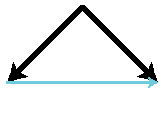
\includegraphics[scale=1.25]{images/Dragon01}
  \hfill
  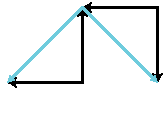
\includegraphics[scale=1.25]{images/Dragon02}
  \hfill
  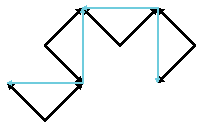
\includegraphics[scale=1.25]{images/Dragon03}
  \hfill
  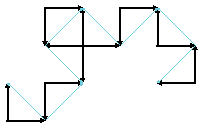
\includegraphics[scale=1.25]{images/Dragon04}
  \caption[The first four iterations of the dragon fractal.]{
    The first four iterations of the dragon fractal.
    The cyan lines give the previous iteration for reference.
  }
  \label{fig:DragonFirst4}
\end{figure}

What makes the dragon fractal different than the Koch Snowflake and similar fractals like the the quadratic curves implementation-wise is that the direction shape flips from one side to another.
Note in the second image of Figure~\ref{fig:DragonFirst4} the first bend is under the its associated line segment whereas the second is above its line segment.
The easiest way for us to control the bend is to alternate the direction of the line segments.
In Figure~\ref{fig:DragonFirst4} each line segment has an arrowhead indicating the orientation of the first and second point with the arrowhead at the second point.
Note that the shape is defined such that the first point of both line segments meet at the right angle.
With the shape defined this way, each iteration is applied to put the bend to the left of the segment with respect to an observer at the first point looking at the second point.

\begin{figure}[tbp]
  \centering
  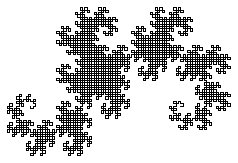
\includegraphics[width=\linewidth]{images/Dragon12}
  \caption{The dragon fractal after 12 iterations.}
  \label{fig:Dragon12}
\end{figure}

Other than reversing the direction of half the line segments, the implementation of the dragon fractal is nearly identical to the Koch Snowflake.

\vtkmlisting{A worklet to generate the dragon fractal.}{DragonFractal.cxx}

\index{dragon fractal|)}

\subsection{Hilbert Curve}

\index{Hilbert curve|(}

For our final example we will look into using our fractal worklet to construct a space-filling curve.
A space-filling curve is a type of fractal that defines a curve that, when iterated to its infinite length, completely fills a space.
Space-filling curves have several practical uses by allowing you to order points in a 2 dimensional or higher space in a 1 dimensional array in such a way that points close in the higher dimensional space are usually close in the 1 dimensional ordering.
For this fractal we will be generating the well-known Hilbert curve.
(Specifically, we will be generating the 2D Hilbert curve.)

The 2D Hilbert curve fills in a rectangular region in space.
(Our implementation will fill a unit square in the [0,1] range, but a simple scaling can generalize it to any rectangle.)
Without loss of generality, we will say that the curve starts in the lower left corner of the region and ends in the lower right corner.
The Hilbert curve starts by snaking around the lower-left corner then into the upper-left followed by the upper-right and then lower-right.
The curve is typically generated by recursively dividing and orienting these quadrants.

To generate the Hilbert curve in our worklet system, we will define our line segments as the connection from the lower left of (entrance to) the region to the lower right of (exit from) the region.
The fractal generation breaks this line to a 4 segment curve that moves up, then right, then back down.
Figure~\ref{fig:Hilbert} demonstrates the Hilbert curve.
(Readers familiar with the Hilbert curve might notice the shape is a bit different than other representations.
Where many derivations derive the Hilbert curve by connecting the center of oriented boxes, our derivation uses a line segment along one edge of these boxes.
The result is a more asymmetrical shape in early iterations, but the two approaches are equivalent as the iterations approach infinity.)

\begin{figure}[htb]
  \centering
  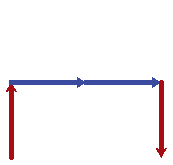
\includegraphics[width=.24\linewidth]{images/Hilbert01}
  \hfill
  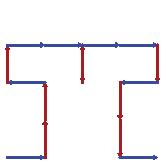
\includegraphics[width=.24\linewidth]{images/Hilbert02}
  \hfill
  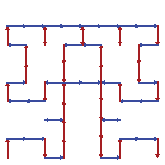
\includegraphics[width=.24\linewidth]{images/Hilbert03}
  \hfill
  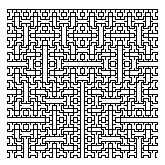
\includegraphics[width=.24\linewidth]{images/Hilbert06}
  \caption[Hilbert curve fractal.]{The first, second, third, and sixth iterations, respectively, of the Hilbert curve fractal.}
  \label{fig:Hilbert}
\end{figure}

Like the dragon fractal, the Hilbert curve needs to flip the shape in different directions.
For example, the first iteration, shown at left in Figure~\ref{fig:Hilbert}, is drawn to the ``left'' of the initial line along the horizontal axis.
The next iteration, the second image in Figure~\ref{fig:Hilbert}, is created by drawing the shape to the ``right'' of the vertical line segments but to the left of the horizontal segments.

Section~\ref{sec:DragonFractal} solved this problem for the dragon fractal by flipping the direction of some of the line segments.
Such an approach would work for the Hilbert curve, but it results in line segments being listed out of order and with inconsistent directions with respect to the curve.
For the dragon fractal, the order and orientation of line segments is of little consequence.
But for many applications of a space-filling curve the distance along the curve is the whole point, so we want the order of the line segments to be consistent with the curve.

To support this flipped shape while preserving the line segment order, we will use a data field attached to the line segments.
That is, each line segment will have a value to represent which way to draw the shape.
If the field value is set to 1 (represented by the blue line segments in Figure~\ref{fig:Hilbert}), then the shape is drawn to the ``left.''
If the field value is set to -1 (represented by the red line segments in Figure~\ref{fig:Hilbert}), then the shape is inverted and drawn to the ``right.''
This field is passed in and out of the worklet using the \textsignature{FieldIn} and \textsignature{FieldOut} tags.

\vtkmlisting{A worklet to generate the Hilbert curve.}{HilbertCurve.cxx}

\index{Hilbert curve|)}


\index{worklet types!creating new|)}
